\documentclass[border=3mm]{standalone}
\usepackage{pgfplots}\pgfplotsset{compat=1.18}
\usepackage{fontspec}\setmainfont{Liberation Sans}
\usepackage{unicode-math}\setmathfont{TeX Gyre DejaVu Math}\newcommand{\Ohm}{Ω}
\usetikzlibrary{arrows.meta}
\definecolor{dunkel}{HTML}{1F3A5F}\definecolor{heiss}{HTML}{E4572E}\definecolor{gruen}{HTML}{2E7D4F}\definecolor{grau}{HTML}{6B6B6B}
\begin{document}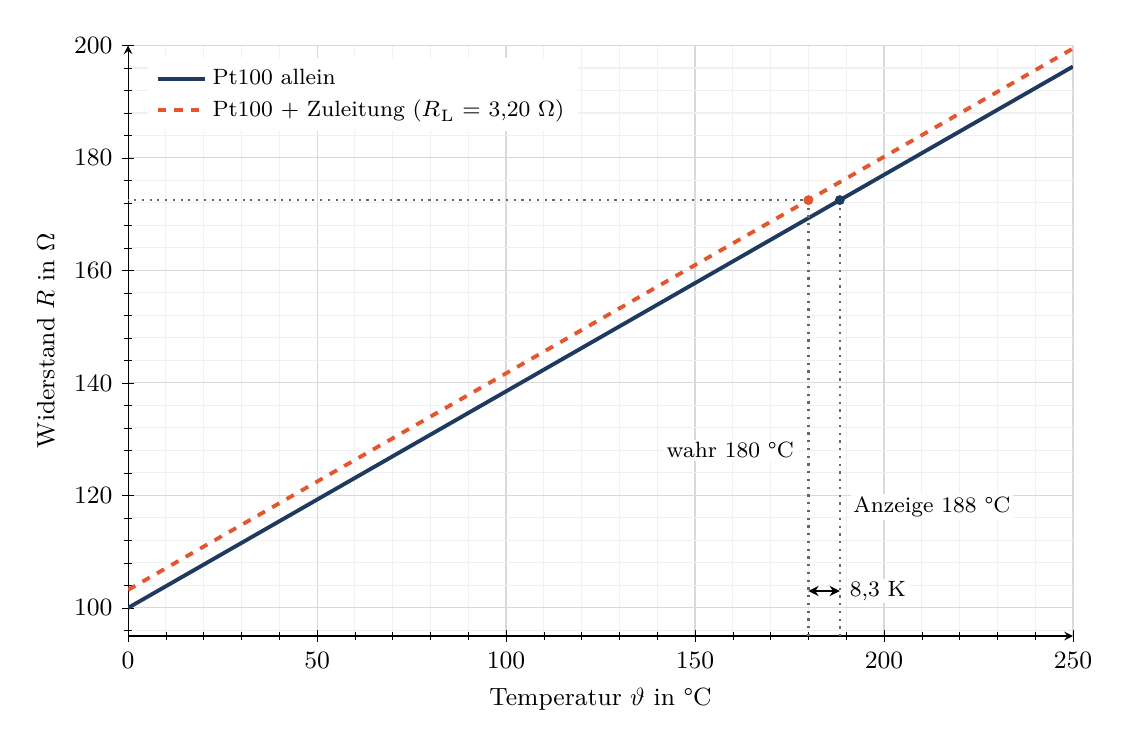
\begin{tikzpicture}
\begin{axis}[width=12cm,height=7.5cm,scale only axis,xmin=0,xmax=250,ymin=95,ymax=200,xlabel={Temperatur $ϑ$ in °C},ylabel={Widerstand $R$ in \Ohm{}},grid=both,grid style={black!15},minor tick num=4,minor grid style={black!6},axis lines=left,tick style={black},/pgf/number format/use comma,/pgf/number format/1000 sep={\,},every axis label/.style={font=\small},tick label style={font=\small},legend cell align=left,xticklabel={\pgfmathprintnumber[assume math mode=true]{\tick}},yticklabel={\pgfmathprintnumber[assume math mode=true]{\tick}},legend style={draw=none,fill=white,font=\footnotesize,at={(0.02,0.98)},anchor=north west},xtick distance=50,ytick distance=20]
\addplot[dunkel,line width=1.4pt,no marks] coordinates {(0,100) (2.5,100.963) (5,101.925) (7.5,102.888) (10,103.85) (12.5,104.812) (15,105.775) (17.5,106.737) (20,107.7) (22.5,108.662) (25,109.625) (27.5,110.587) (30,111.55) (32.5,112.512) (35,113.475) (37.5,114.437) (40,115.4) (42.5,116.362) (45,117.325) (47.5,118.288) (50,119.25) (52.5,120.213) (55,121.175) (57.5,122.138) (60,123.1) (62.5,124.063) (65,125.025) (67.5,125.988) (70,126.95) (72.5,127.913) (75,128.875) (77.5,129.838) (80,130.8) (82.5,131.763) (85,132.725) (87.5,133.688) (90,134.65) (92.5,135.613) (95,136.575) (97.5,137.537) (100,138.5) (102.5,139.463) (105,140.425) (107.5,141.387) (110,142.35) (112.5,143.312) (115,144.275) (117.5,145.238) (120,146.2) (122.5,147.162) (125,148.125) (127.5,149.088) (130,150.05) (132.5,151.012) (135,151.975) (137.5,152.938) (140,153.9) (142.5,154.862) (145,155.825) (147.5,156.787) (150,157.75) (152.5,158.712) (155,159.675) (157.5,160.637) (160,161.6) (162.5,162.562) (165,163.525) (167.5,164.487) (170,165.45) (172.5,166.412) (175,167.375) (177.5,168.338) (180,169.3) (182.5,170.263) (185,171.225) (187.5,172.188) (190,173.15) (192.5,174.113) (195,175.075) (197.5,176.037) (200,177) (202.5,177.963) (205,178.925) (207.5,179.887) (210,180.85) (212.5,181.812) (215,182.775) (217.5,183.738) (220,184.7) (222.5,185.663) (225,186.625) (227.5,187.588) (230,188.55) (232.5,189.513) (235,190.475) (237.5,191.438) (240,192.4) (242.5,193.363) (245,194.325) (247.5,195.288) (250,196.25)};\addlegendentry{Pt100 allein}
\addplot[heiss,line width=1.4pt,dashed,no marks] coordinates {(0,103.204) (2.5,104.166) (5,105.129) (7.5,106.091) (10,107.054) (12.5,108.016) (15,108.979) (17.5,109.941) (20,110.904) (22.5,111.866) (25,112.829) (27.5,113.791) (30,114.754) (32.5,115.716) (35,116.679) (37.5,117.641) (40,118.604) (42.5,119.566) (45,120.529) (47.5,121.492) (50,122.454) (52.5,123.416) (55,124.379) (57.5,125.342) (60,126.304) (62.5,127.267) (65,128.229) (67.5,129.192) (70,130.154) (72.5,131.117) (75,132.079) (77.5,133.042) (80,134.004) (82.5,134.967) (85,135.929) (87.5,136.892) (90,137.854) (92.5,138.817) (95,139.779) (97.5,140.742) (100,141.704) (102.5,142.667) (105,143.629) (107.5,144.591) (110,145.554) (112.5,146.517) (115,147.479) (117.5,148.442) (120,149.404) (122.5,150.367) (125,151.329) (127.5,152.292) (130,153.254) (132.5,154.216) (135,155.179) (137.5,156.142) (140,157.104) (142.5,158.066) (145,159.029) (147.5,159.992) (150,160.954) (152.5,161.916) (155,162.879) (157.5,163.841) (160,164.804) (162.5,165.767) (165,166.729) (167.5,167.691) (170,168.654) (172.5,169.617) (175,170.579) (177.5,171.542) (180,172.504) (182.5,173.467) (185,174.429) (187.5,175.392) (190,176.354) (192.5,177.317) (195,178.279) (197.5,179.242) (200,180.204) (202.5,181.167) (205,182.129) (207.5,183.091) (210,184.054) (212.5,185.017) (215,185.979) (217.5,186.942) (220,187.904) (222.5,188.867) (225,189.829) (227.5,190.792) (230,191.754) (232.5,192.717) (235,193.679) (237.5,194.642) (240,195.604) (242.5,196.567) (245,197.529) (247.5,198.492) (250,199.454)};\addlegendentry{Pt100 + Zuleitung ($R_\mathrm{L}$ = 3,20 \Ohm{})}
\draw[black!60,dotted,line width=0.8pt] (axis cs:180,95) -- (axis cs:180,172.504) -- (axis cs:0,172.504);\fill[heiss] (axis cs:180,172.504) circle (1.8pt);
\draw[black!60,dotted,line width=0.8pt] (axis cs:188.3,172.504) -- (axis cs:188.3,95);\fill[dunkel] (axis cs:188.3,172.504) circle (1.8pt);
\draw[{Stealth[length=1.3mm,width=1.3mm]}-{Stealth[length=1.3mm,width=1.3mm]},line width=0.6pt] (axis cs:180,103) -- (axis cs:188.322,103) node[pos=1,right=0.8mm,font=\footnotesize,fill=white,inner sep=1pt]{8,3 K};
\node[font=\footnotesize,anchor=east,fill=white,inner sep=1pt] at (axis cs:177,128) {wahr 180 °C};
\node[font=\footnotesize,anchor=west,fill=white,inner sep=1pt] at (axis cs:191,118) {Anzeige 188 °C};
\end{axis}
\end{tikzpicture}\end{document}
